\section{BasketView}
\label{basketview}

Der Basket-View bildet alle Menüs und Produkte ab, die zuvor vom Nutzer zu dessen Warenkorb hinzugefügt
worden sind.

Hierfür wird für jede Ware ein \lstinline{Dismissible}-Widget verwendet. Dieses erlaubt dem Nutzer
ungewünschte Menüs und Produkte aus dem Warenkorb entfernt werden.
\cite{flutterDismissible}

\subsection{Dismissible-Widget für Ware}

Mithilfe eines Dismissible-Widets kann der Nutzer einfach seinen Warenkorb verwalten und hinzugefügte
Menüs und Produkte mithilfe eines kurzen Swipes über das Widget wieder entfernen.

Damit dies funktioniert muss einerseits jedes Dismissible-Widget einen \textit{Unique Key} erhalten,
damit die Engine weiß, welches Card-Widget vom Widget-Tree entfernt werden soll.

Andererseits ist eine Implementation der \lstinline{onDismissed}-Funktion erforderlich. In dieser
wird festgelegt, was nach Entfernen eines Dismissibles geschehen soll.\\
In unserem Fall soll das bestimmte Produkt bzw. Menü vom Warenkorb und damit auch vom
\nameref{basketcontroller} entfernt werden und der Gesamtpreis des Warenkorbs aktualisiert werden.

\begin{code}[H]
    \centering
    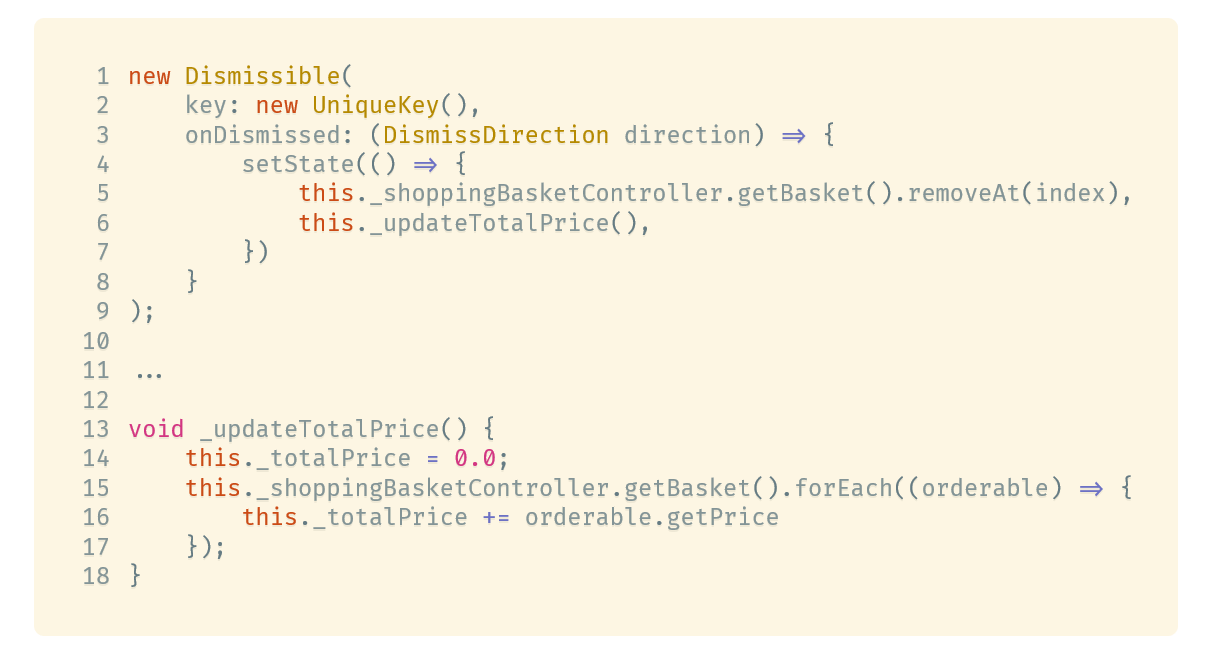
\includegraphics[width=1\textwidth]{images/Client/views/basketview/dismissible.png}
    \vspace{-20pt}
    \caption{Dismissible-Widget im Basket-View mit \lstinline{_updateTotalPrice}-Funktion zum Aktualisieren des Gesamtpreises}
    \label{dismissible}
\end{code}

\subsection{Darstellen des Warenkorbs}

Wie bereits im \nameref{menuview} und \nameref{productview} verwendet, kommt auch hier wieder
das \lstinline{ListView.builder}-Widget zum Einsatz, um für jede Ware im Warenkorb ein 
entsprechendes Dismissble-Widget zu generieren und anzuzeigen.

Der aktuelle Gesamtpreis des Warenkorbs wird mithilfe eines Textfelds auf einem
\lstinline{BottomAppBar}-Widget dargestellt und bei jeder Veränderung der vorübergehend 
gespeicherten Waren aktualisiert, wie in Snippet \ref{dismissible} zu sehen ist.

Um eine Bestellung aufzugeben wird ein \lstinline{FloatingActionButton} an das Bottom-App-Bar-Widget
gebunden, welcher auf Druck ein \lstinline{ModalBottomSheet}-Widget öffnet und die verschiedenen
Kaufoptionen anzeigt.

\begin{figure}[H]
    \centering
    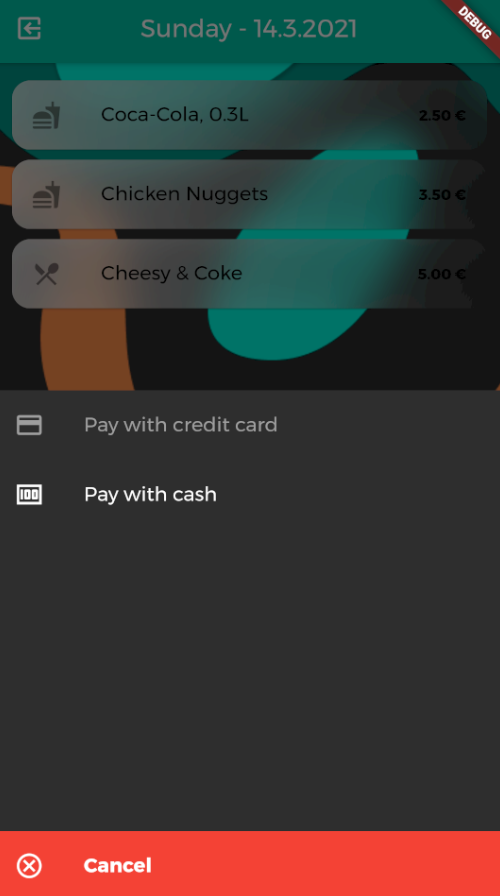
\includegraphics[width=0.40\textwidth]{images/Client/views/basketview/modalSheet.png}
    \caption{Modal-Bottom-Sheet im Basket-View zum Wählen der Bezahloption}
\end{figure}

Ist der Warenkorb des Nutzers leer, so soll als Alternative zu einem leeren List-View-Builder
das Sokka-Logo als Platzhalter angezeigt werden.

\begin{code}[H]
    \centering
    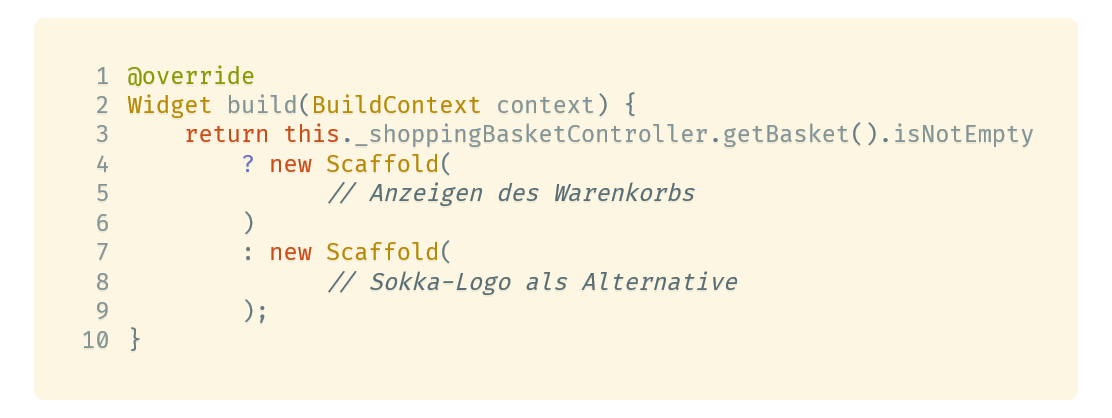
\includegraphics[width=1\textwidth]{images/Client/views/basketview/ternary.png}
    \vspace{-20pt}
    \caption{StaggeredGridView.countBuilder-Widget zum Erzeugen und Darstellen der Product-Tiles}
\end{code}

Dies lässt sich mithilfe obigen Ternary-Operators in der \lstinline{build()}-Funktion des Views
einfach realisieren. Dieser soll abhängig vom Warenkorb zwei verschiedene Scaffolds erzeugen und
führt zu folgendem Resultat:

\begin{figure}[H]
    \centering
    \hfill
    \subfigure[Basket-View mit verschiedenen Waren]{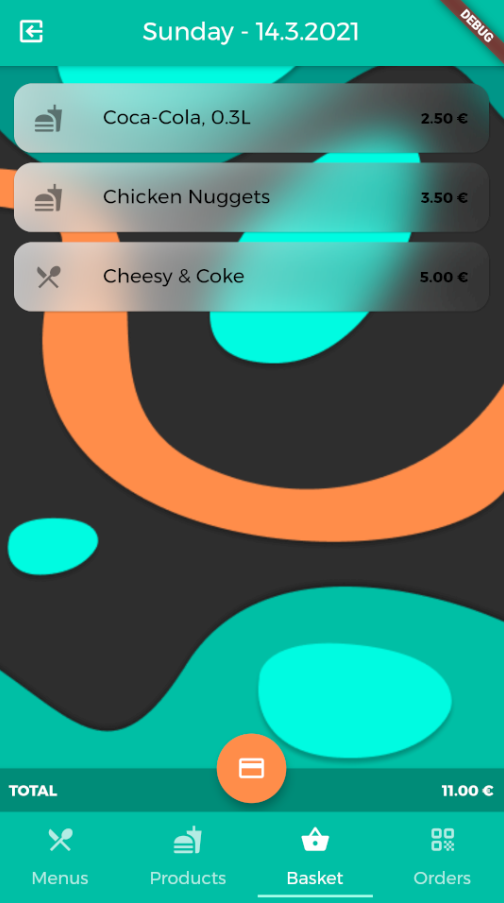
\includegraphics[width=0.4\textwidth]{images/Client/views/basketview/fullBasket.png}}
    \hfill
    \subfigure[Leerer Basket-View]{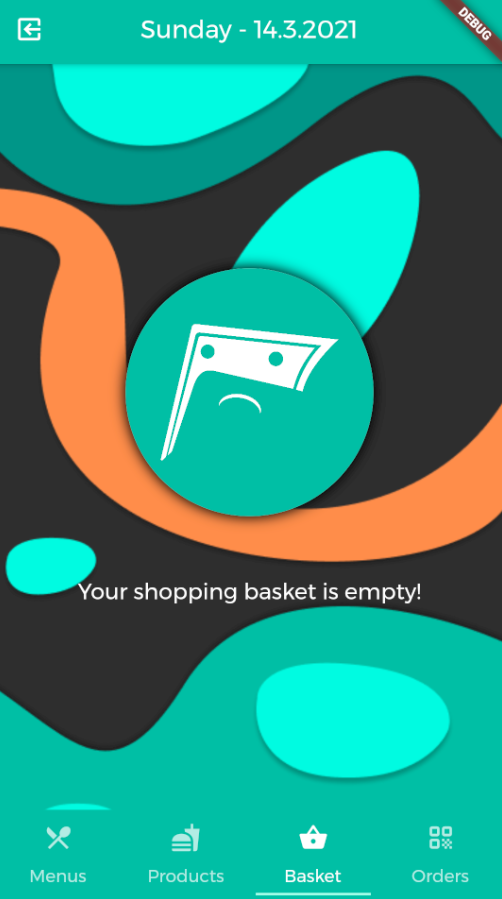
\includegraphics[width=0.4\textwidth]{images/Client/views/basketview/emptyBasket.png}}
    \hfill
    \caption{Basket-View in befüllter und leerer Form}
\end{figure}